\documentclass[sigconf,anonymous,review]{acmart}
\setcopyright{none}
\settopmatter{printacmref=false}
\renewcommand\footnotetextcopyrightpermission[1]{}
\acmConference[WWW '27 -- Draft]{The ACM Web Conference 2027}{May 10--14, 2027}{Dublin, Ireland}
\acmBooktitle{}
\acmDOI{}
\acmISBN{}
\usepackage{amsmath,booktabs}
\setlength{\emergencystretch}{1em}
\newtheorem{theorem}{Theorem}
\newtheorem{proposition}[theorem]{Proposition}
\newtheorem{corollary}[theorem]{Corollary}
\newcommand{\kl}{\operatorname{kl}}
\newcommand{\E}{\mathbb E}
\newcommand{\ind}{\mathbf 1}
\newcommand{\Kor}{K_{\mathrm{or},\alpha}}
\newcommand{\KS}{K_{\mathcal S,\alpha}}
\title[Learning How to Ask in Recommendation]{The Cost of Learning How to Ask in Interactive Recommendation}
\author{Anonymous Author(s)}
\begin{document}
\begin{abstract}
A recommender that asks about a new visitor's preferences may also need to learn which questions yield dependable answers. When this knowledge transfers across several preferences, can learning how to ask become asymptotically free? We study reliable identification of a slot-constrained recommendation slate under two unknown response-reliability levels, group-shared preferred query formats, and finite labelled calibration. We characterize the leading interaction cost through a joint information program and compare it with an oracle that knows the preferred formats but not their accuracies. Our main result gives a necessary and sufficient condition for equality with this oracle: the smallest sharing group determines whether learning the formats incurs a positive first-order cost. Without calibration at the logarithmic confidence scale, equality holds exactly when the known partition contains a single group. The result identifies a structural limit on amortizing elicitation effort. The channel assumptions require separate validation for natural-language users and LLM simulators.
\end{abstract}
\begin{CCSXML}
<ccs2012><concept><concept_id>10002951.10003227.10003351</concept_id><concept_desc>Information systems~Recommender systems</concept_desc><concept_significance>500</concept_significance></concept></ccs2012>
\end{CCSXML}
\ccsdesc[500]{Information systems~Recommender systems}
\keywords{Preference elicitation, interactive recommendation, query reliability, calibration, sample complexity}
\maketitle

\section{Introduction}
An online shopping assistant can ask what a visitor wants and still receive an answer that is hard to trust. A visitor may understand how a device will be used more readily than the specifications that describe it. Work on conversational recommendation has consequently explored questions about item usage as an alternative to direct attribute questions~\cite{kostric2021}. The choice of question becomes part of preference acquisition: the system must learn both what the visitor prefers and how to obtain a dependable expression of that preference.

Learning a useful way to ask is most valuable when it can be reused. Several requirements may share an accessible form of expression, while a different domain may call for another form. A platform with limited historical calibration then faces a concrete budget question: how much additional interaction is needed because the reliable form is initially unknown? A reliable personalized slate requires resolving the visitor's preferences, but some early interactions also serve to identify the observation channel. Counting these two roles separately is difficult because the same answer can inform both.

Preference elicitation already connects query selection to recommendation quality~\cite{guo2010}. Unknown feedback quality is also well established: crowdsourced ranking learns annotator quality alongside rankings~\cite{chen2013}, and preference models can jointly estimate utilities and rationalities~\cite{yamagata2024}. These results motivate our question rather than settle it. We ask for an explicit boundary between settings where learning the reliable form changes the leading interaction cost and settings where it does not. Our comparison grants both learner and oracle the same finite calibration; the oracle knows only which form is better in each group. Giving it the reliability levels as well would answer a different question.

We study this boundary in a deliberately restricted recommendation problem. Each fixed slate slot has two candidates, and the best choice in one slot does not depend on choices in other slots. This makes identifying the entire optimal slate equivalent to recovering its binary preferences. For the response channel, two unknown accuracy levels are shared globally, while the identity of the better form is shared within a known preference group. Conditional independence and this sharing structure are assumptions to be checked in an application, not properties implied by natural-language interaction.

Our main result is a smallest-group criterion: whether the learner matches the format-informed oracle depends on the least amount of within-group sharing, not the average group size. The full partition can still determine the size of a positive gap. Without calibration at the logarithmic confidence scale, a single sharing group is necessary and sufficient for the first-order premium to vanish. We build on controlled sensing and structured pure exploration~\cite{deshmukh2019,degenne2019,garivier2016}; our contribution is an explicit cost boundary for the shared-channel problem. It separates two sources of user burden: learning preferences and learning their reliable expression.

\section{Reliable Slate Elicitation}
\paragraph{A recommendation objective.}
There are $d$ fixed slots, each containing two candidates indexed by $-1,+1$. The visitor has fixed preferences $\theta\in\{-1,+1\}^d$. For a slate $a\in\{-1,+1\}^d$, let
\begin{equation}\label{eq:utility}
 U(a;\theta)=\sum_{j=1}^d w_j\ind\{a_j=\theta_j\},\qquad w_j>0.
\end{equation}
We require the entire returned slate to be optimal with probability at least $1-\delta$, rather than optimize average ranking quality.
\begin{proposition}[Decision equivalence]\label{prop:slate}
Under~\eqref{eq:utility}, identifying the optimal slate with error at most $\delta$ has the same query complexity as recovering $\theta$ with that error bound, under the same observation interface.
\end{proposition}
\begin{proof}
The unique optimal slate is $a^*=\theta$. Either procedure therefore supplies the output of the other without another observation or any additional cost.
\end{proof}
This equivalence uses independent slot feasibility and positive weights. In an arbitrary catalogue, different preference vectors can induce the same optimal item; recovering every preference may then be unnecessary, and our lower bound does not automatically apply to top-item identification.

\paragraph{Unknown reliability with sharing.}
A known partition $\mathcal S$ groups preferences into sets $S_1,\ldots,S_G$, with $k_g=|S_g|$. Query $(j,m)$ asks about the \emph{same} binary choice in form $m\in\{1,2\}$. Group $g$ has an unknown better form $z_g$. A fresh answer satisfies
\begin{equation}\label{eq:channel}
 \Pr(Y=\theta_j\mid j,m,h)=
 \begin{cases}p,&m=z_{g(j)},\\q,&m\ne z_{g(j)},\end{cases}
\end{equation}
where $h=(\theta,z,p,q)$ and $1/2\le q<p\le1-\eta$, for known $\eta\in(0,1/2)$. The two levels are unknown and common across groups. Answers are conditionally independent given $h$. Both forms have access to the same task evidence; changing the underlying decision or revealing extra evidence would change the experiment.

Before interaction, the learner receives $M_\delta$ independent labelled observations from each of $\operatorname{Bern}(p)$ and $\operatorname{Bern}(q)$. Their stream identities reveal high versus low reliability, not the current $z$ or $\theta$. Write $R_\delta=\log(1/\delta)$ and $M_\delta/R_\delta\to\alpha<\infty$. Obtaining such labelled references requires a calibration design; unlabelled historical conversations are not equivalent resources.

Each online answer costs one interaction. Optionally, one interaction can report $z_g$ with known accuracy $s_g\in(1/2,1)$, independently of the past. It has finite distinguishing information $\kappa_g=\kl(s_g,1-s_g)$. A perfect report is treated separately. A unit-cost action returning the whole profile is outside this single-answer interface.

\paragraph{An information-matched oracle.}
Policies must be uniformly $\delta$-correct over the stated parameter domain, with error probability including calibration randomness. Let $C_\delta(h)$ be the infimum expected online cost. The oracle receives $z$, but retains the same unknown $p,q$, preferences, calibration and costs. Total acquisition cost is $2M_\delta+C_\delta(h)$; the common offline cost must not be hidden when reporting savings.

\section{An Exact Boundary for the Cost of Learning Formats}
Let $D(r,x)=\kl(r,x)$ denote Bernoulli KL divergence. For action $e$, let $P_h^e$ be its binary answer law, and let $\operatorname{Alt}(h)$ contain states with a different $\theta$. Define $D_0(h,h')=D(p,p')+D(q,q')$. The information coefficient is
\begin{equation}\label{eq:program}
\begin{split}
 K(h,\alpha)=\min_{x\ge0}\;&\sum_e x_e\\
 \text{s.t. }&\alpha D_0(h,h')+\sum_e x_eD(P_h^e\Vert P_{h'}^e)\ge1\\
 &\hspace{38mm}\text{for every }h'\in\operatorname{Alt}(h).
\end{split}
\end{equation}
The infima use the closure $1/2\le q'\le p'\le1-\eta$. Optional type-report actions are included in $e$ when available.

\paragraph{Calibration-aware joint tracking.}
We specialize information tracking to this channel. A forced exploration schedule supplies $\Omega(\sqrt t)$ observations of every task stream. Their empirical means estimate the sign from the sum of the two answer probabilities, and the group type from the larger sign-oriented mean; pooled good/other means estimate $p,q$. At exploitation rounds, solve~\eqref{eq:program} at these estimates with $\alpha_\delta=M_\delta/R_\delta$, and track the minimizing action proportions. Forced observations remain part of the evidence; no early type estimate is permanently trusted.

For stopping, use the full joint likelihood $L_t$ of calibration and online answers. Define $\ell_t(\vartheta)=\sup_{z,p,q}\log L_t(\vartheta,z,p,q)$ over the continuous rate domain, and let $\widehat\theta_t$ maximize it. Return $\widehat\theta_t$ only when
\begin{align}\label{eq:stop}
 \ell_t(\widehat\theta_t)-\max_{\vartheta\ne\widehat\theta_t}\ell_t(\vartheta)&\ge\beta(t,\delta),\\
 \beta(t,\delta)&=R_\delta+2\log(M_\delta+1)\notag\\
 &\quad+\sum_{e\text{ online}}\log(N_e(t)+1).\notag
\end{align}
Here $N_e(t)$ counts action $e$ before stopping. This is a joint test of the desired recommendation, allowing different channel explanations on either side. It does not replace uncertain reliability by a fixed estimated channel.

\begin{theorem}[Leading interaction cost]\label{thm:cost}
For fixed $d,\mathcal S,\eta$ and any fixed true $h$ satisfying~\eqref{eq:channel},
\[
 C_\delta(h)=K(h,\alpha)R_\delta+o(R_\delta).
\]
The upper bound is attained by an ideal real-arithmetic exploration-and-tracking policy with vanishing actual optimization errors. It is pointwise, not uniform in growing $d$ or vanishing reliability gaps.
\end{theorem}
\begin{proof}[Proof outline]
The stopped-transcript KL equals the reference contribution $M_\delta D_0$ plus expected action counts times their KL divergences. Data processing for the correct-output event gives $\kl(1-\delta,\delta)$; normalizing yields~\eqref{eq:program}. This offline/online decomposition also appears in offline-data best-arm identification~\cite{agrawal2023}, with a different observation structure.

For the error bound, integrate an unrestricted Bernoulli law for each stream against a uniform Beta prior, obtaining $Q_t$. Streamwise maximum likelihood is at most $(N_e+1)$ times this mixture. Under the true state, $Q_t/L_t(h)$ is a mean-one martingale initialized \emph{before} calibration. An incorrect output in~\eqref{eq:stop} forces this ratio above $1/\delta$, so Ville's inequality bounds its probability by $\delta$.

For expected cost, use a vanishing estimation grid, actual feasibility/optimality errors tending to zero independently of $\delta$, and tracking discrepancy $O(\sqrt t)$. Same-type alternatives flipping one preference force a positive online information margin. Centering calibration and online likelihood increments together, compact rate nets and forced-sample concentration yield
$\Pr_h(\tau>t)\le Ct^A e^{-c\sqrt t}$ for $t\ge(K+\varepsilon)R_\delta$, uniformly over sufficiently small $\delta$. Summing this tail gives the expected-cost upper bound. Optimizer-set tracking avoids assuming a unique optimizer; the oracle's uniqueness below is a separate structural fact.
\end{proof}

The joint program is important even when the partition is known. Changing the candidate levels $p',q'$ changes answer distributions in \emph{every} group at once. The least distinguishable wrong explanation can therefore couple groups through those levels. Adding independent known-channel costs for each group would miss this effect; finite calibration restricts the explanations without eliminating them.

The coefficient is invariant to the true sign and form labels; write it as $\KS$. Its oracle counterpart has a scalar description. Put
\[
 F_k(r,x)=D(r,1-x)+(k-1)D(r,x).
\]
Let $a_\alpha>0$ be the unique solution of
\begin{equation}\label{eq:oracle}
 \inf_{1/2\le v\le u\le1-\eta}
 \{\alpha[D(p,u)+D(q,v)]+a_\alpha F_d(p,u)\}=1.
\end{equation}
\begin{proposition}[Oracle allocation]\label{prop:oracle}
$\Kor=da_\alpha$. Its unique optimal first-order task allocation assigns $a_\alpha$ to the better form of every coordinate and zero to all other actions.
\end{proposition}
\begin{proof}[Proof outline]
Symmetrize coordinates. With per-coordinate good/other counts $a,b$, the constraint is the infimum of $\alpha[D(p,u)+D(q,v)]+aF_d(p,u)+bF_d(q,v)$. At a minimizer $(u_*,v_*)$ in~\eqref{eq:oracle}, $u_*\le p$ and $v_*=\min(q,u_*)$. Crucially, $A=F_d(p,u_*)>B=F_d(q,v_*)$: when $u_*\le q$, $F_d(r,u_*)$ strictly increases between $q$ and $p$; otherwise $A\ge(2p-1)\log[u_*/(1-u_*)]>D(q,1-q)=B$. This fixed alternative rules out $a+b\le a_\alpha$ with $b>0$. Symmetrization preserves average other-form mass, so it vanishes in every optimum.

An under-sampled coordinate then violates its sign-flip constraint whenever $u_*>1/2$, forcing equal good-form counts. For $d=2,\alpha=0,u_*=1/2$, its constraint has negative derivative in $u$, so moving slightly above $1/2$ gives the violation. For $d=1$ there are no unequal counts. Finally the left side of~\eqref{eq:oracle} increases continuously from zero to infinity with $a_\alpha$, proving existence and uniqueness of the root.
\end{proof}

Define $k_{\min}=\min_g k_g$ and
\begin{align}
 w_k&=\max\left\{\tfrac12,\frac{\alpha q+a_\alpha[1+(k-2)p]}{\alpha+ka_\alpha}\right\},\label{eq:w}\\
 \Gamma_k(\alpha)&=\alpha D(q,w_k)+a_\alpha F_k(p,w_k).\label{eq:gamma}
\end{align}
\begin{theorem}[Smallest-group boundary]\label{thm:boundary}
With or without finite-information type reports,
\begin{equation}\label{eq:boundary}
 \boxed{\KS=\Kor\quad\Longleftrightarrow\quad\Gamma_{k_{\min}}(\alpha)\ge1.}
\end{equation}
Otherwise the extra expected online cost has strictly positive leading coefficient $\KS-\Kor$.
\end{theorem}
\begin{proof}
Equality requires the oracle's unique allocation; any positive type-report cost would already make it more expensive. It suffices to test this allocation against unknown-type alternatives. Additional wrong signs only increase divergence because candidate accuracies are at least $1/2$, so retain one flipped preference.

If this preference lies within reversed-type groups containing $l$ coordinates, their fitted other-form rate is $v$; the remaining rate can be fitted at $u=p$. The constraint reduces exactly to
\[
 \inf_{v\ge1/2}\{\alpha D(q,v)+a_\alpha F_l(p,v)\}=\Gamma_l(\alpha).
\]
Its minimizer is $w_l\le p$, so the order constraint is respected. Since $F_{l+1}(p,v)=F_l(p,v)+D(p,v)$, this value is nondecreasing in $l$. The smallest nonempty reversed-type set is a group of size $k_{\min}$.

If the flipped preference is outside the reversed-type set, replacing the latter's $D(p,v)$ terms by $D(p,u)$ only lowers information at a minimizer with $v\le u\le p$. The resulting constraint is the oracle constraint and is at least one. Thus the least information at the oracle allocation is $\min\{1,\Gamma_{k_{\min}}\}$. Feasibility proves equality; otherwise attainment of the closed information program and oracle uniqueness give a strict cost gap.
\end{proof}

\begin{corollary}[No logarithmic-scale calibration]\label{cor:zero}
If $\alpha=0$, the first-order premium vanishes exactly when $G=1$.
\end{corollary}
\begin{proof}
Let $I_k(p)=\inf_{1/2\le x\le1-\eta}F_k(p,x)$. Then $a_0=1/I_d(p)$ and $\Gamma_k(0)=I_k(p)/I_d(p)$. We have $I_1=D(p,1/2)$ and $I_2=2I_1$. For $k\ge2$, $I_k=k[H(p-(2p-1)/k)-H(p)]$, where $H$ is binary entropy; strict concavity gives strict increase in $k$. Hence the criterion holds exactly at $k_{\min}=d$.
\end{proof}

\section{Implications and Model Checks}
\begin{figure}[t]
 \centering
 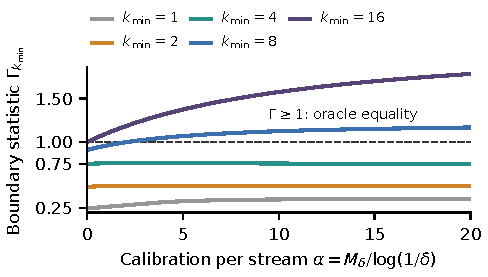
\includegraphics[width=\linewidth]{figures/sharing_boundary.pdf}
 \caption{Boundary diagnostic for $d=16,p=.85,q=.60,\eta=.05$. Curves evaluate~\eqref{eq:gamma} for equal-size partitions; values at least one imply zero first-order premium. Calibration is measured per reference stream. These are numerical evaluations of the theorem, not measured user accuracies.}
 \label{fig:boundary}
\end{figure}
The boundary distinguishes reuse from overhead. At the parameters of Figure~\ref{fig:boundary} and $\alpha=4$, partitions $(8,8)$ and $(1,15)$ have the same average group size. Yet $\Gamma_8\simeq1.051$ and $\Gamma_1\simeq.318$: the first partition has zero leading premium and the second a positive one. A large group cannot compensate for an isolated preference. Grouping unrelated questions by name does not create this sharing structure. More calibration cannot increase either learner or oracle cost separately; their difference need not be monotone.

Type reports provide a useful control. Noisy reports can reduce a positive premium; they leave~\eqref{eq:boundary} unchanged. If reports are \emph{perfect}, at most $G$ interactions reveal all types. This cost does not scale with $R_\delta$, so the leading premium vanishes. Learning the format remains nontrivial when self-reports convey only finite information.

The response assumptions require their own validation. In a small exploratory audit of two synthetic profile worlds and paired private representations, a local Qwen3.6-35B-A3B service answered 65/128 balanced diagnostic choices correctly and selected the first displayed candidate 103/128 times. Candidate identities and order were independently crossed. This is a development diagnostic, not a human study, and does not establish the shared symmetric channel. We retain it as a boundary check rather than use simulator errors as evidence for reliable elicitation.

\section{Scope and Conclusion}
Reliable preference acquisition has a cost beyond learning the preferences themselves. For the stated slate and channel model, we characterize that cost and show exactly when sharing removes its leading term. The result suggests evaluating elicitation interfaces by their sharing structure and calibration requirements, alongside dialogue length and recommendation quality.

The assumptions remain substantial: fixed preferences, a known valid partition, common accuracy levels, labelled references and fresh conditional independence. Position bias, persistent errors, unknown grouping and general catalogue ranking require different analysis. The ideal theorem also does not certify an implementation with fixed numerical floors. These limits define concrete next questions for recommendation research rather than an established account of natural users.

\bibliographystyle{ACM-Reference-Format}
\bibliography{references}
\end{document}
